\subsection{Background simulations}

\begin{frame}{Background sources}
\ilclogo
The main sources of background:
\begin{columns}
 \begin{column}{0.55\textwidth}
  \begin{itemize}
    \item Pair background
    \item Bhabha scattering
    \item \textgamma \textgamma $\rightarrow$ hadrons
    \item Neutrons from the beam dumps
    \item Background from Final-Focus system (beam halo collimators, muon spoilers)
  \end{itemize}
 \end{column}
 \begin{column}{0.45\textwidth}
 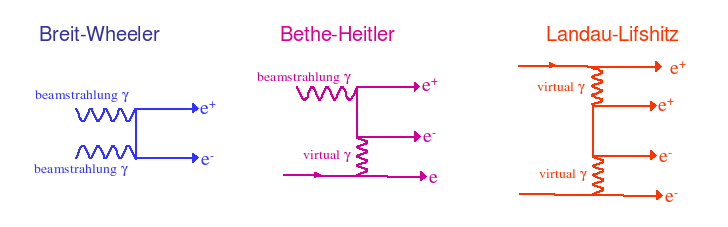
\includegraphics[height=0.2\textheight]{figures/beamstrahlung_processes.png}\\
 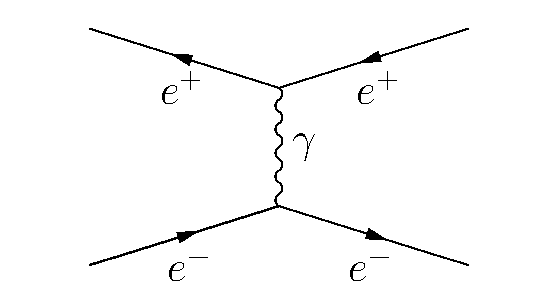
\includegraphics[height=0.15\textheight]{figures/bhabha_scattering.pdf} 
 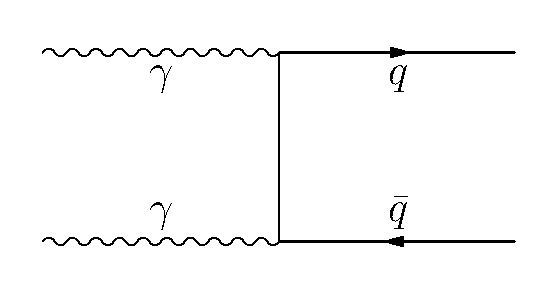
\includegraphics[height=0.15\textheight]{figures/gammagamma_hadrons.pdf}
 \end{column}
\end{columns}

\vspace*{0.5cm}
\visible<2->{
$\Rightarrow$So, if the ILC is supposed to see such clean signals, the question is:\\
\vspace*{0.5cm}
With all these background sources, how many background events do the detectors get?
}
\end{frame}


